Consider the problem of a star of mass $M_*=M_\odot$ (where 
$M_\odot=\SI{1.99e30}{\kilogram}$ surrounded by a planet of 
$M_p=10^{-3} M_\odot$. At time $t=0$ the planet is located at 
coordinates $(1,0,0)$ in units of AU$=\SI{1.496e11}{\meter}$. The 
planet's velocity is $(0,0.5,0)$ in units of the Kepler velocity at the 
that location, which is 
$v_K(1\textnormal{ AU})=\SI{2.98e4}{\meter\per\second}$
\\

\subsection{Solve the Kepler orbit of this planet using numerical
    integration with the leapfrog algorithm. Find an appropriate 
    time step. Plot the result for the first few orbits.
} \ \\
    The leapfrog algorithm reads:
    \begin{align}
        v_{i+1/2}&=v_i+a(x_i)\cdot\frac{\Delta t}{2} \\
        x_{i+1/2}&=x_{i}+v_{i+1/2}\cdot\frac{\Delta t}{2}
    \end{align}
    It can be implemented using the following iterative python function: \\
    \begin{lstlisting}
        # define helper functions
        norm = lambda x: np.sqrt(sum([i**2 for i in x]))
        a = lambda x: -G * M_star * x / norm(x)**3

        def leapfrog_integrate(x_0, v_0, steps):
            x, v = x_0, v_0
        
            # single integration step
            def leapfrog_step(x, v): 
                new_v = v + a(x) * dt / 2
                new_x = x + new_v * dt / 2
                return new_x, new_v
        
            xs, vs = [], []
            # iterate, then return position and velocity
            for _ in range(steps):
                x, v = leapfrog_step(x, v)
                xs.append(x)
                vs.append(v)

            return xs, vs\end{lstlisting} 
    After playing around a little bit with the parameters, it seems like 
    a step-size of $\Delta t=\SI{1e-2}{}$ leads to a good trade-off between 
    accuracy and integration time. With this step-size, one orbit takes 
    approximately 5350 integration steps.
    \begin{figure}[h!]
        \centering
        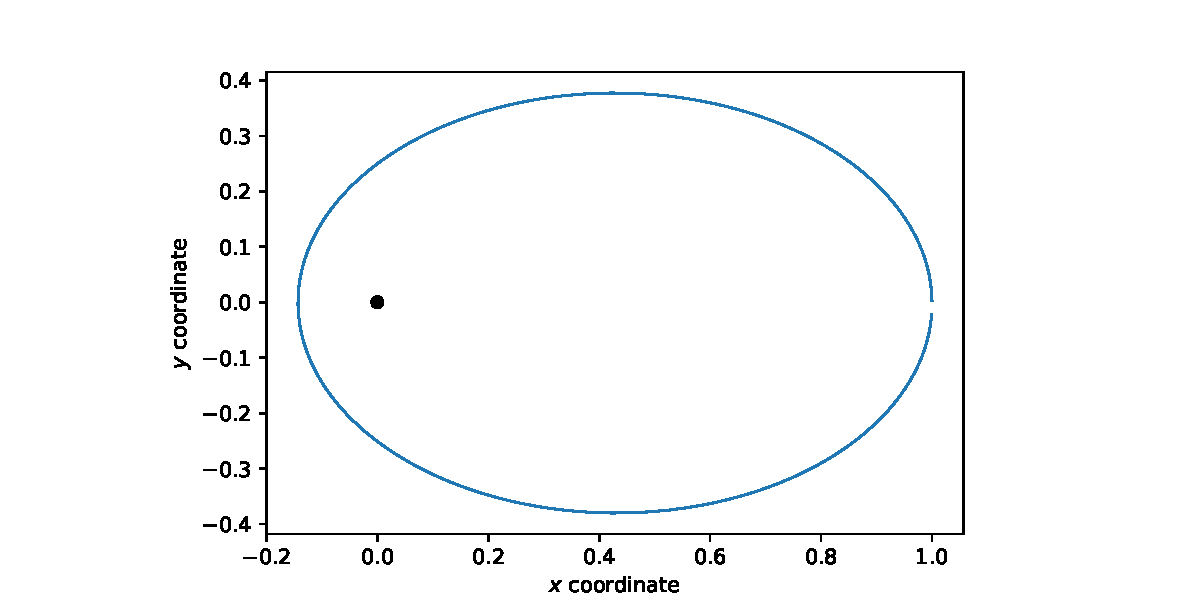
\includegraphics[width=\textwidth]{./figures/task1_1_orbit_lf.pdf}
        \caption{Trajectory of the planet after approximately one orbit
            ($N=5350$, $dt=10^{-2}$).
        }
    \end{figure} \ \\ 

\newpage
\subsection{Now integrate for 100 orbits and see how the orbit behaves.}
    As can be seen below, the orbiting planet does not come back to exactly the 
    same spot after each time it circles the star, which is due to the discrete
    nature of the simulation (e.g. finitely small $\Delta t$). The errors add 
    up after each orbit, and the simulated planet starts precessing around the 
    star.
    \begin{figure}[h!]
        \centering
        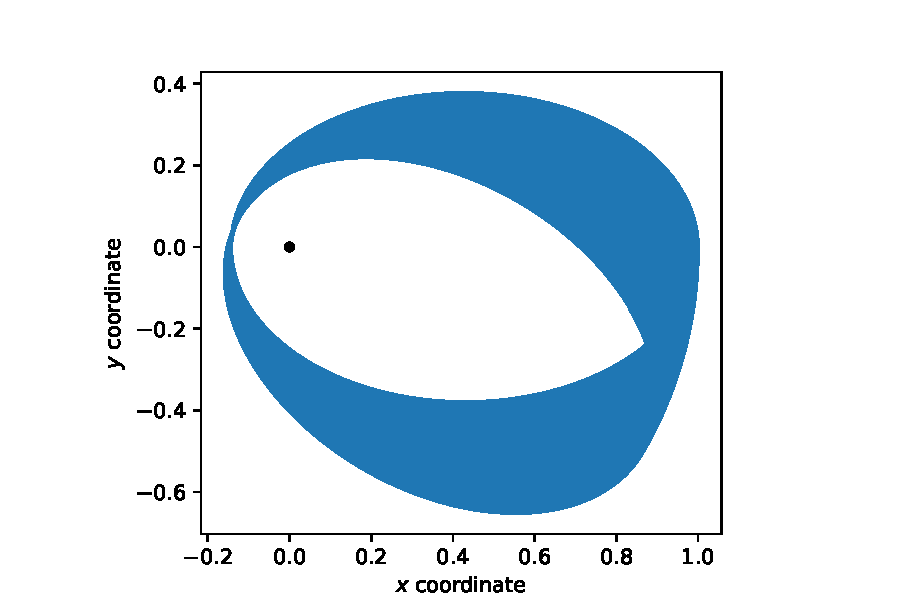
\includegraphics[width=\textwidth]{./figures/task1_1_orbit_lf_100.pdf}
        \caption{Trajectory of the planet after approximately 100 orbits
            ($N=10^5$, $dt=10^{-2}$).
        }
    \end{figure}

\newpage
\subsection{Repeat this with the RK2 and RK4 algorithms and see how the 
    system behaves. Discuss the difference to the leapfrog algorithm.
} \ \\
    To implement the Runge-Kutta solver, we can use the following function: \\
    \begin{lstlisting}
        def rk_integrate(x_0, v_0, dt, steps, order=2):
        
            # define derivative function
            def f(t, y):
                x = np.array(y[:3])
                v = np.array(y[3:])
        
                dv = a(x) * dt
                dx = v * dt
                return list(dx) + list(dv)
        
            y_0 = list(x_0) + list(v_0)
            # initialize integrator (either Rk2 or Rk4)
            if order == 2:
                rk_integrator = RK23(
                    f, t_0, y0=y_0, t_bound=dt*steps, first_step=dt, max_step=dt
                )
            elif order == 4:
                rk_integrator = RK45(
                    f, t_0, y0=y_0, t_bound=dt*steps, first_step=dt, max_step=dt
                )
        
            # iterate and return
            ys = []
            for _ in range(steps):
                rk_integrator.step()
                ys.append(rk_integrator.y)
        
            return np.array(ys)\end{lstlisting}
    \begin{itemize}
        \item energy is bound from above and below in leapfrog, in 
            RK2 the energy grows over time
        \item angular momentum is strictly conserved in leapfrog, not shown 
            but provable
        \item energy error grows linearily (on average) in RK4, 
            but much slower as RK2, and for long times it's lower than 
            for leapfrog
    \end{itemize}
    % \begin{figure}[h!]
    %     \centering
    %     \begin{minipage}{.5\linewidth}
    %       \centering
    %       \subfloat[2nd order Runge-Kutta]{
    %         \label{:a}
    %         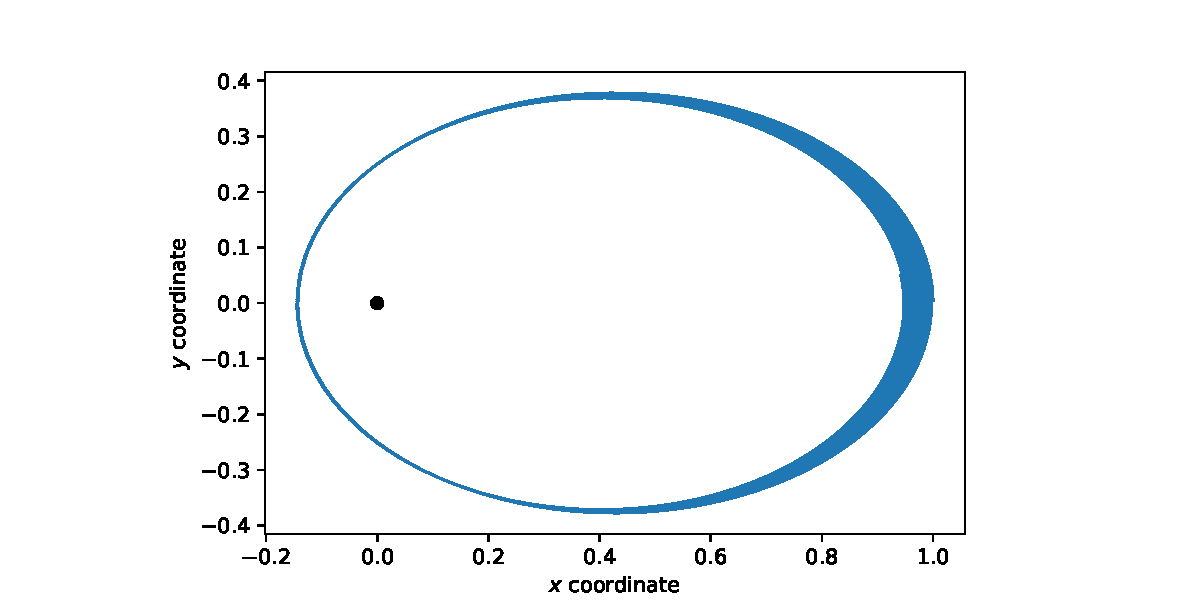
\includegraphics[scale=.5]{./figures/task1_1_orbit_rk2.pdf}
    %       }
    %     \end{minipage}%
    %     \begin{minipage}{.5\linewidth}
    %       \centering
    %       \subfloat[4th order Runge-Kutta]{
    %         \label{:b}
    %         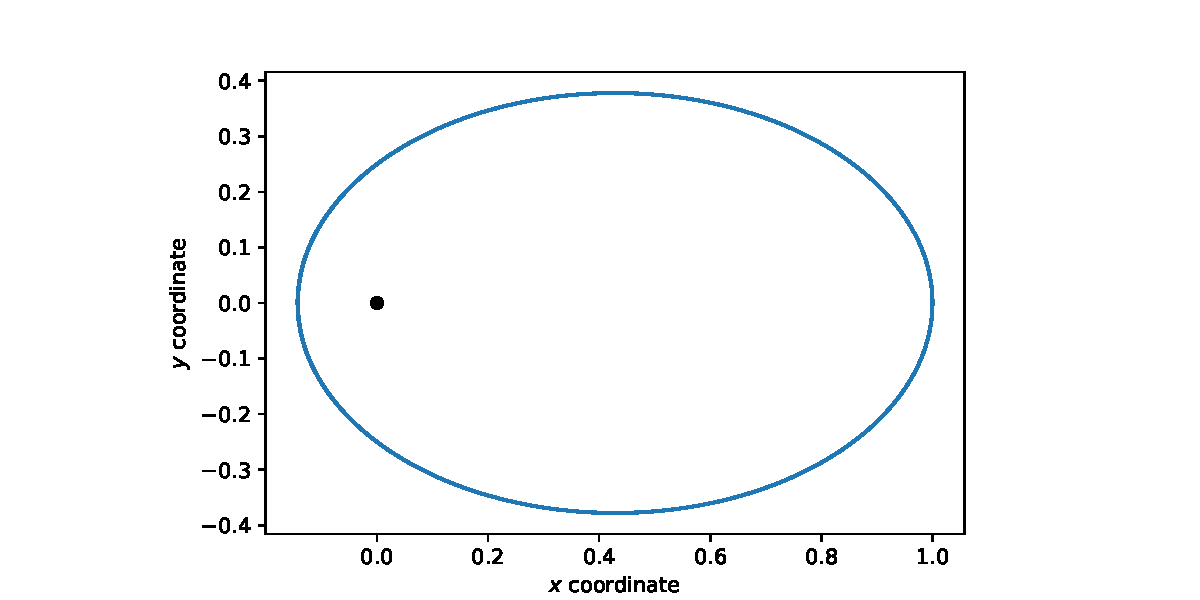
\includegraphics[scale=.5]{./figures/task1_1_orbit_rk4.pdf}
    %       }
    %     \end{minipage}
    % \end{figure} \ \\
    \newpage \noindent
    As can be seen in the plots below, energy is not conserved in Rk2, as the 
    planet "spirals" inwards toward the star.
    \begin{figure}[h!]
        \centering
        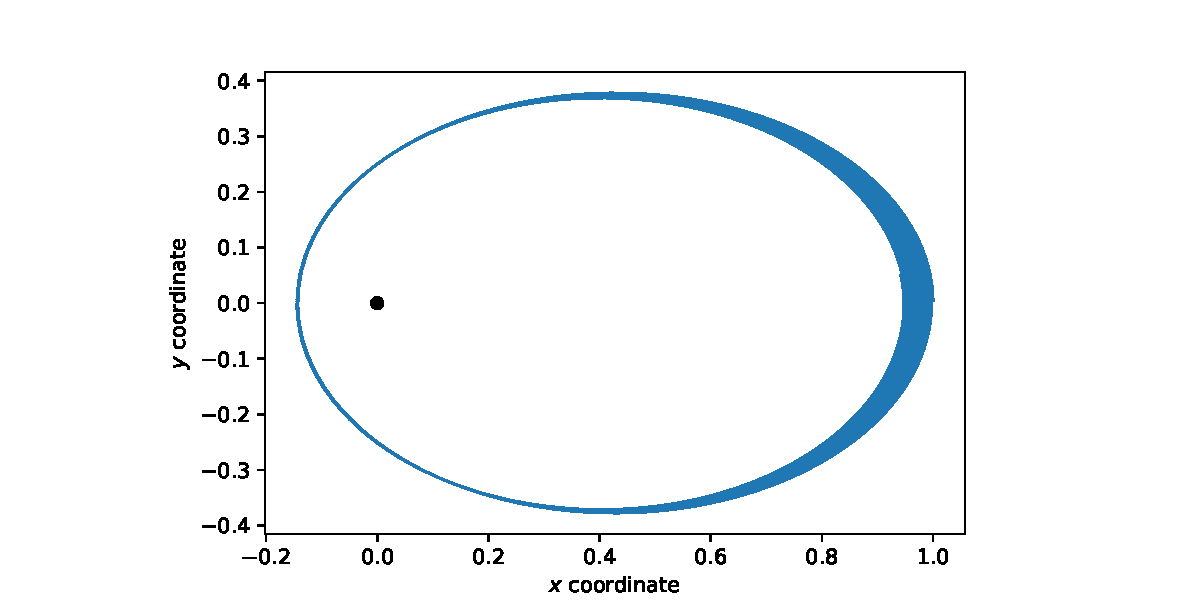
\includegraphics[width=\textwidth]{./figures/task1_1_orbit_rk2.pdf}
        \caption{2nd order Runge-Kutta algorithm}
    \end{figure} \ \\ 
    \begin{figure}[h!]
        \centering
        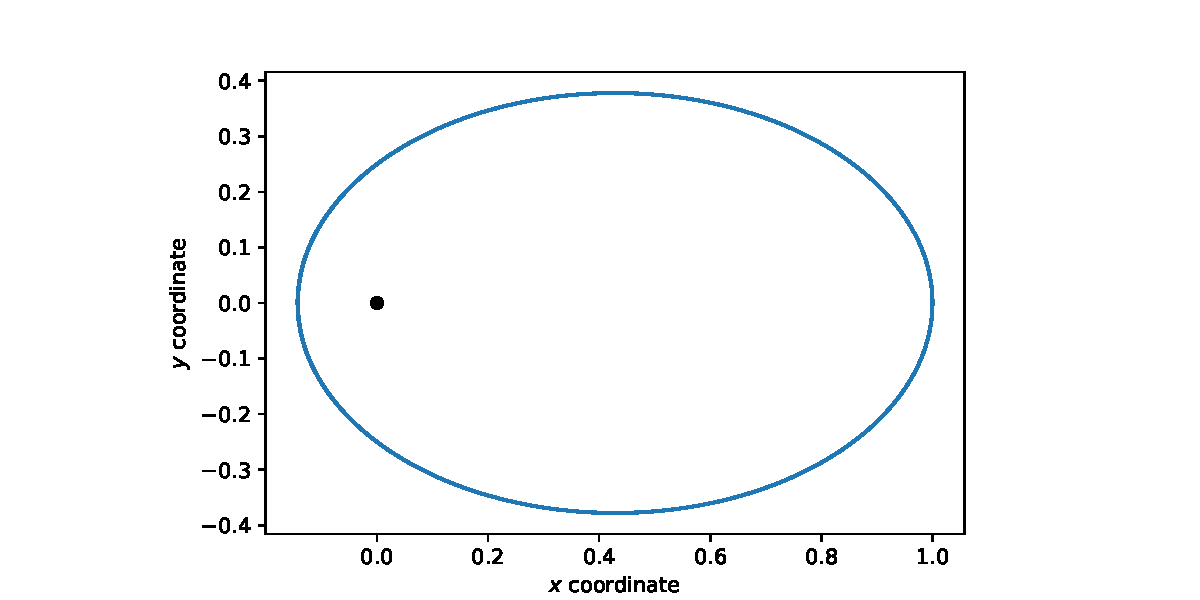
\includegraphics[width=\textwidth]{./figures/task1_1_orbit_rk4.pdf}
        \caption{4th order Runge-Kutta algorithm}
    \end{figure} \ \\ 

    \newpage
    \subsection{Plot the time evolution of the relative error 
        of the total energy and the time evolution of the total kinetic
        energy of the system.}
    \begin{figure}[h!]
        \centering
        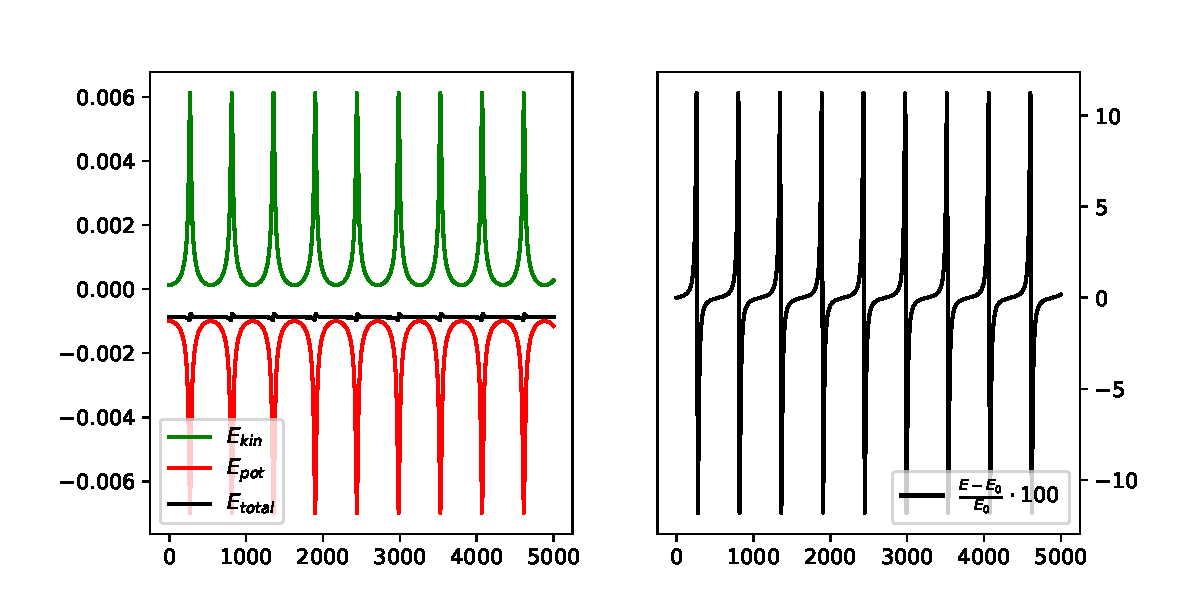
\includegraphics[width=\textwidth]{./figures/task1_1_energies_lf_test.pdf}
        \caption{total energy balance as well as relative energy error plotted 
            vs. time for leapfrog solver}
    \end{figure} \ \\ 
    \begin{figure}[h!]
        \centering
        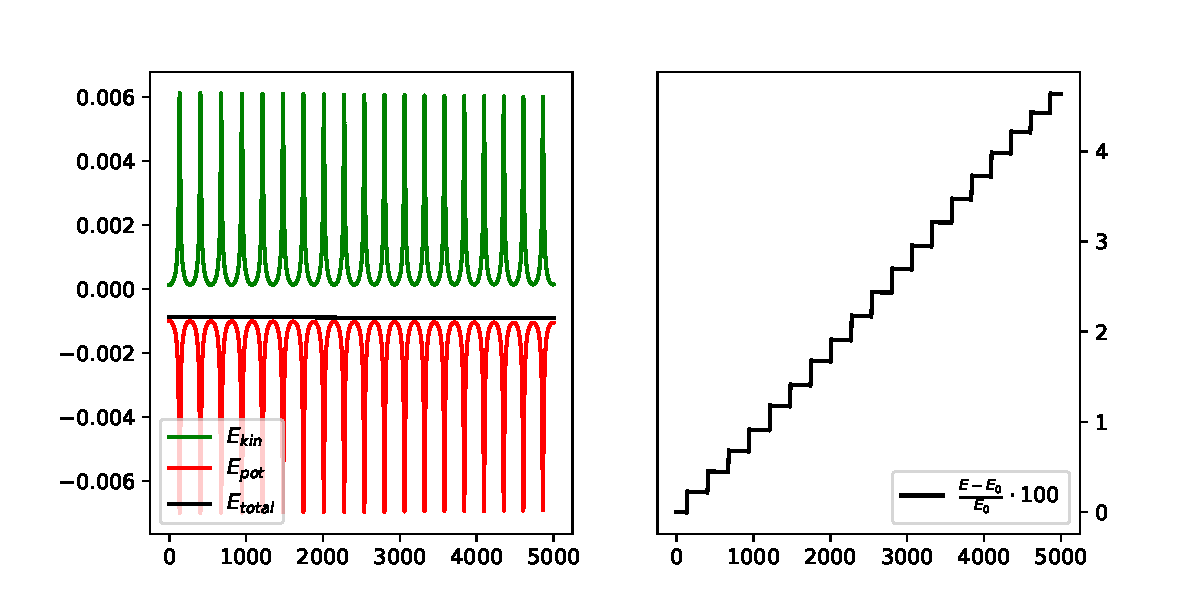
\includegraphics[width=\textwidth]{./figures/task1_1_energies_rk2.pdf}
        \caption{total energy balance as well as relative energy error plotted 
            vs. time for second-order Runge-Kutta}
    \end{figure} \ \\ 
    \begin{figure}[h!]
        \centering
        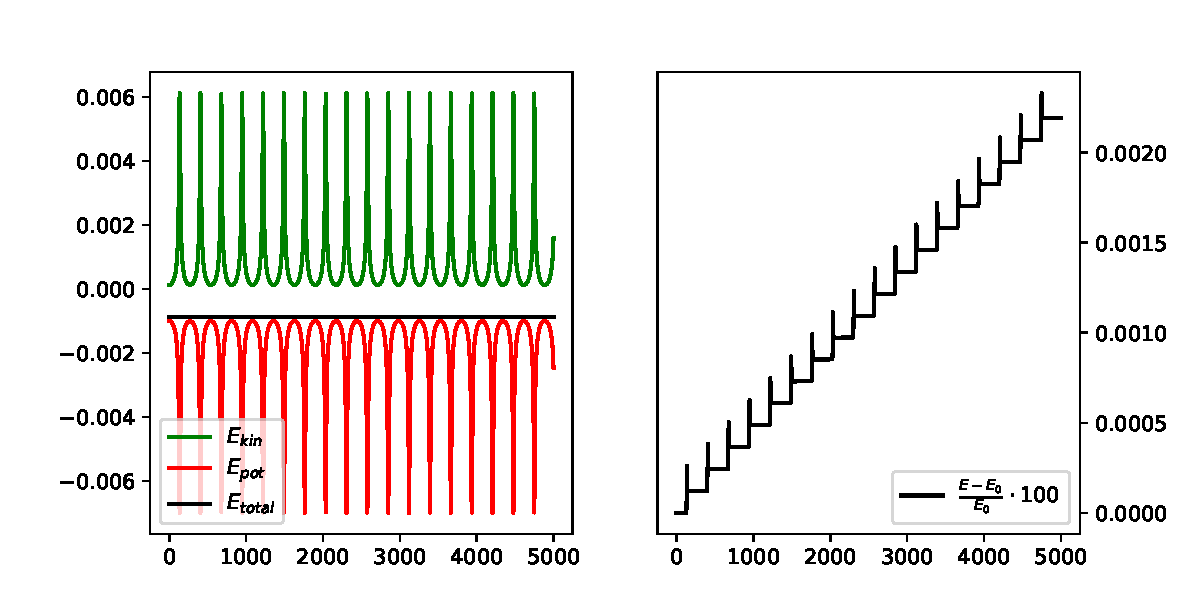
\includegraphics[width=\textwidth]{./figures/task1_1_energies_rk4.pdf}
        \caption{total energy balance as well as relative energy error plotted 
            vs. time for fourth-order Runge-Kutta}
    \end{figure} \ \\ 
   \begin{comment}
    \begin{figure}[h!]
        \centering
        \begin{minipage}{.5\linewidth}
          \centering
          \subfloat[evolution of angular momentum]{
            \label{:a}
            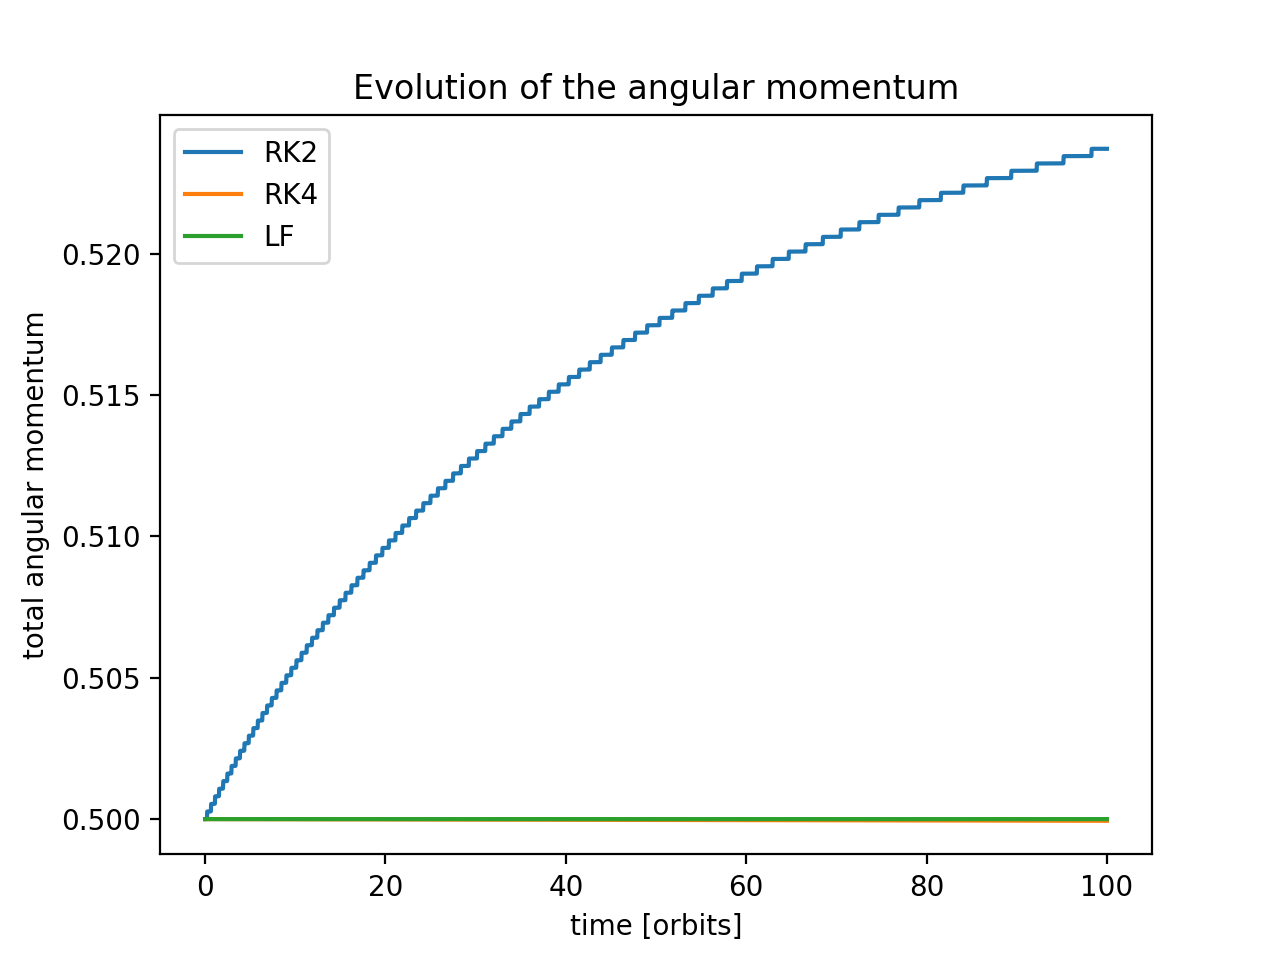
\includegraphics[scale=.55]{./k/angularMom100.png}
          }
        \end{minipage}%
        \begin{minipage}{.5\linewidth}
          \centering
          \subfloat[evolution of energy]{
            \label{:b}
            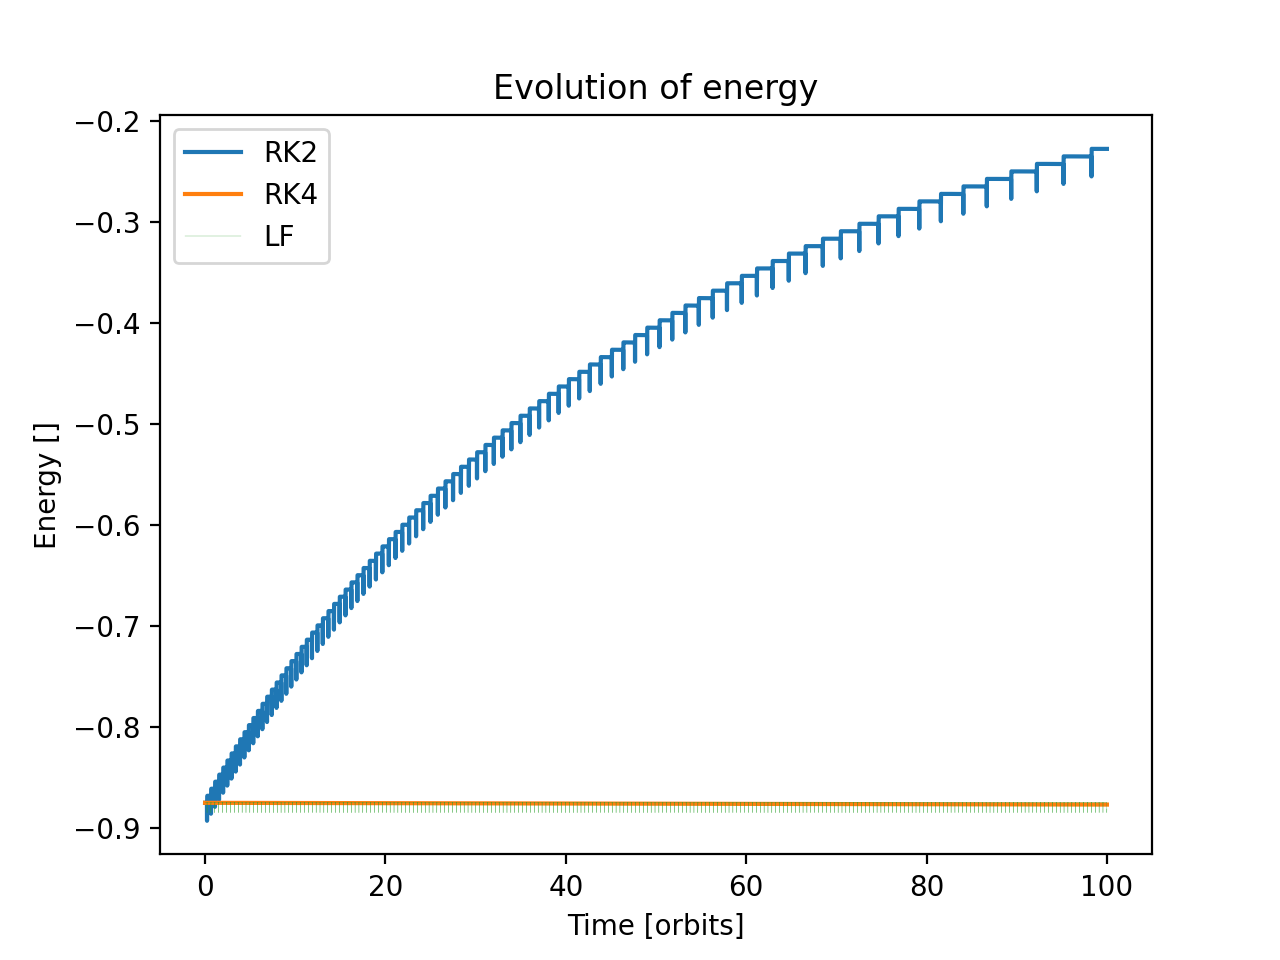
\includegraphics[scale=.55]{./k/energy100.png}
          }
        \end{minipage}
        \caption{Energy and angular momentum for leapfrog, Rk2 and Rk4. 
            The quantities are not conserved when using the second order 
            Runge-Kutta scheme, but fourth order and leapfrog do respect 
            the conservation laws.}
    \end{figure} \ \\

\end{comment}
